\documentclass[conference]{IEEEtran}
\IEEEoverridecommandlockouts
\usepackage[utf8]{inputenc}
\usepackage[T1]{fontenc}
\usepackage{amsmath,amssymb,amsfonts}
\usepackage{graphicx}
\usepackage{booktabs}
\usepackage{multirow}
\usepackage{xcolor}
\usepackage[colorlinks=false,pdfborder={0 0 0}]{hyperref}

\begin{document}

\title{Beyond Subword Fluency: Semantic Coherence\\ Modeling for Zero-Day Wordlist DGA Detection}

\author{\IEEEauthorblockN{Walid Mahmood}
\IEEEauthorblockA{\textit{Department of Computer Science and Engineering}\\
\textit{BRAC University}, Dhaka, Bangladesh\\
walid.mahmood@g.bracu.ac.bd}}

\maketitle

\begin{abstract}
Wordlist-based Domain Generation Algorithms (DGAs) evade character-statistical detection by concatenating legitimate dictionary words---\texttt{sugarmouse.com}, \texttt{travel-orange-river.info}---producing domains whose letter-level statistics (vowel structure, character runs, digit content) sit far closer to benign traffic than to algorithmic DGAs. Published detection scores for this class are routinely measured under protocols that place the malware's own dictionary in the training set, leaving the true zero-day generalization floor unmeasured. This paper introduces a strict, leak-free Leave-Families-Out (LFO) benchmark on 1.3M domains spanning 43 DGA families, in which six validation families guide checkpoint selection and five completely unseen families---three of them wordlist---are evaluated exactly once. We propose \textbf{Dual-Branch Coherent}, a 0.73M-parameter architecture that couples a character BiLSTM and a FastText word-sequence BiLSTM through a learnable gate with an explicit 6-dimensional pairwise-cosine coherence vector, ablated against an identical 4.10M-parameter backbone without the vector and against a fine-tuned ModernBERT-Base (149M) on the same data. Under fully blind conditions, ModernBERT achieves the best overall F1 (0.7372 vs.\ 0.6799) and benign specificity (95.56\%) yet collapses to 14.15\% recall on the unseparated dictionary family \texttt{matsnu}, where the proposed 0.73M model reaches 17.60\% (+24.4\% relative) with 204$\times$ fewer parameters; a soft-voting ensemble of the two combines these strengths into the strongest deployment profile (100\% recall on unseen non-wordlist families, 94.88\% benign specificity, 34.25\% wordlist macro-recall). Together, these results expose a structural ``subword fluency'' blind spot in transformer tokenization and show that an explicit, computed semantic signal repairs exactly that failure mode.
\end{abstract}

\begin{IEEEkeywords}
Domain Generation Algorithm (DGA), wordlist DGA, zero-day generalization, semantic coherence, FastText, ModernBERT, BiLSTM, DNS security, benchmark methodology
\end{IEEEkeywords}

\section{Introduction}
Algorithmic domain generation is a primary mechanism by which botnets (e.g., Conficker, Mirai, Gameover Zeus) evade static IP and domain blocklists: the operator and infected hosts independently compute large pools of candidate rendezvous domains. Classical DGAs emit pseudo-random strings (e.g., \texttt{rqwzx817m.net}) that are readily flagged by classifiers over Shannon entropy, vowel--consonant ratios, and character n-grams. In response, malware authors deploy \emph{wordlist-based} DGAs (Matsnu, Ngioweb, Pizd, Suppobox, Gozi), which draw tokens from embedded English dictionaries and concatenate them. Plohmann et al.~\cite{plohmann2016} measured that wordlist families exhibit markedly lower character entropy than all other DGA categories---low enough to fall \emph{below} typical benign entropy---which is precisely why entropy- and n-gram-based detectors fail against them.

The only property separating a legitimate compound domain (\texttt{fishing-gear.com}) from a dictionary DGA (\texttt{sugar-claim-mouse.com}) is \emph{semantic}: whether the constituent words plausibly co-occur. This signal is invisible to character statistics but recoverable from frozen pretrained word embeddings, and it can be computed without ever observing the malware's vocabulary.

This paper is motivated by two gaps in how wordlist-DGA detection is currently evaluated.

\subsubsection*{Gap 1: dictionary leakage in published evaluation}
The strongest published results on this problem class~\cite{leyva2026} train on eight wordlist families---including \texttt{matsnu}, \texttt{suppobox}, and \texttt{manuelita}---and report generalization on the three families held out (\texttt{bigviktor}, \texttt{ngioweb}, \texttt{pizd}). A model that has seen a family's dictionary does not learn ``dictionary DGA'' in general; it memorizes that malware's vocabulary. A botnet operator rotates dictionaries with one line of code, and a defense that depends on having seen the list defends against yesterday's malware. Under a protocol in which the test families are never observed, the same architecture class collapses (Section~\ref{sec:results}).

\subsubsection*{Gap 2: the subword fluency blind spot}
Subword tokenizers (BPE, WordPiece) segment concatenated dictionary words into frequent, grammatical fragments. To a pretrained transformer, \texttt{sugarmouse} appears as fluent brand language; self-attention over high-frequency subwords produces a high language-plausibility score and a benign verdict. We show this is a structural property of the architecture class rather than a data-volume artifact, and that an explicit semantic-coherence feature repairs exactly this failure mode.

\subsubsection*{Contributions}
\begin{enumerate}
\item \textbf{A blind zero-day benchmark for wordlist DGAs.} A strict Leave-Families-Out protocol over 43 DGA families plus benign traffic (1,259,799 training domains; 19,998 frozen test domains), with model selection on held-out validation wordlist families and a single one-shot evaluation on five completely unseen families, checked against confirmed literature anchors~\cite{drichel2022,leyva2026}.
\item \textbf{Two designed architectures, evaluated as an ablation pair.} Dual-Branch Coherent (0.73M parameters) injects an explicit 6-dimensional FastText pairwise-cosine coherence vector into a gated dual-sequence backbone; Dual-Branch v3 (4.10M) is the identical backbone without the vector, isolating the coherence signal from raw capacity.
\item \textbf{A head-to-head transformer comparison on identical data.} A fine-tuned ModernBERT-Base~\cite{modernbert2024} (149M) trained on the same 1.26M-domain split, enabling a defensible efficiency/generality analysis rather than a borrowed baseline.
\item \textbf{Deployment-oriented findings.} An ensemble analysis identifying the operating point suitable for Security Operations Centers (SOCs), an accuracy-per-parameter efficiency analysis, and a fully stated list of threats to validity.
\end{enumerate}

\section{Related Work}
\subsubsection*{Feature-engineered detection}
Early systems extracted structural, temporal, and lexical statistics from passive DNS (EXPOSURE~\cite{bilge2011}, Pleiades~\cite{antonakakis2012}); FANCI~\cite{schuppen2018} classified domains with a random forest over hand-crafted features. Woodbridge et al.~\cite{woodbridge2016} introduced character-level LSTM classifiers. These approaches presuppose the entropy separation that wordlist DGAs violate.

\subsubsection*{Character-level models and the wordlist blind spot}
Lison and Mavroeidis~\cite{lison2017} trained a character GRU jointly across 61 families with a strong aggregate F1 (0.971); their per-family table shows Matsnu recall of only 0.158---among the worst in all families---attributed to data scarcity against a 1,300+-word vocabulary. The failure persists at the architecture level: given enough examples a character model can absorb wordlist structure, but for the families that matter it rarely has them.

\subsubsection*{Semantic approaches}
Koh and Rhodes~\cite{koh2018} fed frozen ELMo embeddings to a small classifier, stripping TLDs and segmenting labels with a Zipfian dynamic-programming segmenter---both choices adopted here. Their model reached 89.5\% detection on Matsnu with \emph{thirty labeled examples} at a 1:1,000 false-positive rate, and verified the model flagged Matsnu domains built from unseen words. Our work asks the strictly harder question: how far does the semantic signal carry with \emph{zero} exposure to the target family?

\subsubsection*{Adversarial wordlist generation}
CharBot~\cite{peck2019} demonstrated that minimal character substitutions of real registered domains suffice to evade state-of-the-art DGA classifiers while producing benign-looking strings. Adversarially generated families of this kind are included in our training wordlists for robustness, and they sharpen the threat model: detectors must generalize not only to unseen dictionaries but to dictionaries designed against them.

\subsubsection*{Evaluation methodology}
Drichel et al.~\cite{drichel2022} established the zero-day reference point: under leave-one-cluster-out evaluation across DGArchive families, the best context-free detector achieves 19.444\% median F1. Cebere et al.~\cite{cebere2024} meta-analyzed 38 detection papers and found per-family difficulty and sample requirements vary enormously, cautioning against generalist protocols. Leyva La O et al.~\cite{leyva2026} benchmarked pretrained transformers (LLaMA~3.2, Gemma~3, ModernBERT, DomBertUrl) on wordlist DGAs; their strongest zero-shot figures (80.9\% F1, ModernBERT; 84.6\%, DomBertUrl) were measured with eight wordlist families in training and on their held-out trio (\texttt{bigviktor}, \texttt{ngioweb}, \texttt{pizd}). UMUDGA~\cite{zago2020dib,zago2020cose} supplies the majority of our corpus.

\subsubsection*{Positioning}
Across these lines, prior semantic approaches either replace the character pathway entirely~\cite{koh2018} or fine-tune a single pretrained transformer without an explicit lexical branch~\cite{leyva2026}; the strongest zero-day baselines aggregate all DGA families rather than isolating the wordlist subset~\cite{drichel2022}; and no prior work, to our knowledge, evaluates an explicit dual-branch (character + frozen-semantic) architecture with a \emph{computed} coherence signal under fully family-blind conditions on wordlist DGAs.

\section{Threat Model and Problem Statement}
We target the following operational scenario: an enterprise or resolver-side detector, trained on historical DGA families, must classify domains from a \emph{wordlist family it has never observed in any form}---not in training, not in validation, not in feature engineering. The adversary controls the embedded dictionary and can rotate it at will; the detector may only rely on properties shared by \emph{all} artificial dictionary concatenations.

Three structural facts define the difficulty:
\begin{enumerate}
\item \textbf{Letter-statistics convergence.} In the training corpus, dictionary DGAs match benign traffic on essentially every letter-level statistic---vowel ratio 0.35 vs.\ 0.36, digit ratio 0.01 vs.\ 0.02, maximum consonant runs 3.3 vs.\ 2.7---while pseudorandom DGAs are far away on all three (0.23, 0.08, 6.3; Table~\ref{tab:lexical}). What separates dictionary DGAs from benign traffic is \emph{length} (15.6 vs.\ 10.3 characters), which also confounds per-character entropy (3.20 vs.\ 2.81 bits). A detector can therefore fit ``long, letter-benign domains are wordlist DGAs'' on the families it has seen---a rule that breaks when an unseen family's dictionary shifts the length profile. This is precisely the classical models' validation$\to$test collapse in Section~\ref{sec:results}.
\item \textbf{Subword fluency.} Subword tokenizers render unseparated concatenations as fluent text, defeating pretrained-language-model intuitions of legitimacy (Section~\ref{sec:inversion}).
\item \textbf{Class asymmetry.} Non-wordlist (algorithmic) DGAs sit far outside natural-language phonotactics and are nearly saturated by all learned models (93--100\% recall in our benchmark); high non-wordlist scores are an inherent property of the problem, not evidence of generalization. The research frontier is the wordlist subset.
\end{enumerate}

\begin{table}[t]
\centering
\caption{Lexical characterization of the training corpus (200{,}000-domain sample, seed 42; mean $\pm$ std). Letter-level statistics place dictionary DGAs next to benign traffic, not next to algorithmic DGAs.}
\label{tab:lexical}
\footnotesize
\setlength{\tabcolsep}{5pt}
\begin{tabular}{@{}lccc@{}}
\toprule
 & Benign & Pseudorandom & Dictionary \\
\midrule
SLD length (chars) & 10.3 $\pm$ 4.5 & 13.4 $\pm$ 5.5 & 15.6 $\pm$ 5.8 \\
Entropy (bits) & 2.81 $\pm$ 0.51 & 3.16 $\pm$ 0.39 & 3.20 $\pm$ 0.38 \\
Vowel ratio & 0.36 $\pm$ 0.12 & 0.23 $\pm$ 0.14 & 0.35 $\pm$ 0.09 \\
Digit ratio & 0.02 $\pm$ 0.08 & 0.08 $\pm$ 0.17 & 0.01 $\pm$ 0.06 \\
Max consonant run & 2.7 $\pm$ 1.2 & 6.3 $\pm$ 3.8 & 3.3 $\pm$ 1.2 \\
\bottomrule
\end{tabular}
\end{table}

\section{Benchmark Design}
\subsection{Corpus}
We merge three public sources (full provenance and audit in the repository): \textbf{UMUDGA}~\cite{zago2020dib,zago2020cose} (50 DGA families plus benign), the wordlist-DGA release accompanying~\cite{leyva2026} (five families absent from UMUDGA: \texttt{charbot}, \texttt{deception}, \texttt{manuelita}, \texttt{bigviktor}, \texttt{ngioweb}), and \textbf{Alexa Top-1M / Tranco} benign domains. Multi-variant families (e.g., \texttt{gozi\_gpl/luther/nasa/rfc4343}) are collapsed to a single label before splitting, so no variant of a family can straddle splits. Because the two DGA sources overlap (e.g., \texttt{pizd} is ~100\% string-identical between them), deduplication operates on exact domain strings, not family names; post-merge cross-split exact matches were re-verified as zero.

\subsection{Preprocessing}
All domains are reduced to second-level domains (SLDs) via \texttt{tldextract} (e.g., \texttt{mail.google.co.uk} $\to$ \texttt{google}), lowercased, exact-FQDN deduplicated, non-ASCII discarded, and length-bounded ($3 \le L \le 64$), retaining 99.99\% of rows. The character vocabulary (38 characters plus four special tokens) is built strictly from the training partition; measured out-of-vocabulary rate is zero on all splits. The EDA suite in the repository quantifies why SLD isolation is necessary rather than assumed: raw-FQDN entropy systematically overstates DGA randomness because the fixed TLD suffix dilutes the label's own statistics, and digit/hyphen ratios measured on raw strings are dominated by formatting artifacts that vanish after processing. A dot-frequency unit test (which must fall from 6.66\% to exactly 0.0000\%) is included as an executable check of the pipeline.

\subsection{Leave-Families-Out partitioning}
Table~\ref{tab:split} summarizes the split. Design decisions and their rationale:

\begin{table}[t]
\centering
\caption{Leave-Families-Out split composition.}
\label{tab:split}
\footnotesize
\setlength{\tabcolsep}{4pt}
\begin{tabular}{@{}lrrp{2.2cm}@{}}
\toprule
Split & Total & DGA/Benign & Families \\
\midrule
Train & 1{,}259{,}799 & 629{,}899 / 629{,}900 & 32 (26 non-WL, 6 WL) \\
Val-Unseen & 23{,}998 & 11{,}999 / 11{,}999 & 6 held-out (3 WL, 3 non-WL) \\
Test-Unseen & 19{,}998 & 10{,}000 / 9{,}998 & 5 zero-day (3 WL, 2 non-WL) \\
\bottomrule
\end{tabular}
\end{table}

\textbf{Wordlist families remain in training (six of nine).} An earlier design held out every wordlist family; it was rejected because it permits the shortcut ``word-like structure $\Rightarrow$ benign,'' since benign domains are word-like too. Keeping \texttt{gozi}, \texttt{rovnix}, \texttt{nymaim}, \texttt{banjori}, \texttt{charbot}, \texttt{deception} in training forces the model to learn what distinguishes \emph{malicious} dictionary concatenations from legitimate ones, while the transfer question is measured on families whose dictionaries are entirely unseen.

\textbf{\texttt{pizd} is test-only} because it is one of only three families against which the strongest published ceiling~\cite{leyva2026} was genuinely measured; training on it would destroy the one clean comparison point. \textbf{\texttt{manuelita}} (a known-difficult family) \textbf{is a validation-time diagnostic} rather than a blind test case---a deliberate derisking trade-off, disclosed in Section~\ref{sec:limitations}. \textbf{\texttt{matsnu}} is retained as the headline hard case: it concatenates words \emph{without} delimiters and was part of the ceiling study's training set, so any score on it is computed under a strictly harder condition than that study attempted.

\subsection{Imbalance handling and checkpoint criterion}
Training contains 26 non-wordlist families (${\sim}510$K domains) versus 6 wordlist families (${\sim}120$K), an 80/20 volume imbalance inherent to family counts. We neutralize it at training time: a weighted sampler enforces ${\sim}1{:}1$ wordlist/non-wordlist composition per mini-batch, and every model is checkpointed on \texttt{val\_wordlist\_macro\_recall}---macro recall over the three \emph{held-out} validation wordlist families---with a non-wordlist recall floor (0.60) as an eligibility guardrail. The checkpoint metric is deliberately not a blended aggregate, which could reward a model whose wordlist performance stagnates. Validation families are used repeatedly (that is their purpose); test families are evaluated exactly once, after all decisions are frozen. All pipelines fix seed 42.

\section{Architectures}
\subsection{Proposed: Dual-Branch Coherent (0.73M parameters)}
The model (Fig.~\ref{fig:arch}) has three signal paths fused by a learnable gate.

\textbf{Character branch.} The SLD is embedded (64-d) and encoded by a BiLSTM with 128 hidden units per direction, $h_{\text{char}} \in \mathbb{R}^{256}$.

\textbf{Word branch.} The SLD is segmented with \texttt{wordninja} (Zipfian-frequency dynamic programming) into tokens $[w_1,\dots,w_k]$, each embedded in a \emph{frozen} FastText 300D table~\cite{bojanowski2017} (the \texttt{.bin} model, so rare tokens and segmentation errors still receive subword-composed vectors), then encoded by a BiLSTM (128 per direction), $h_{\text{word}} \in \mathbb{R}^{256}$. Frozen embeddings follow~\cite{koh2018}: they force the model to use general lexical--semantic structure rather than letting gradient descent find a character-statistical shortcut.

\textbf{Explicit 6-D coherence vector.} For all token pairs $(w_i, w_j)$, $1 \le i < j \le k$, let $s_{ij} = \cos(e(w_i), e(w_j))$ and $S = \{s_{ij}\}$. The vector is
\begin{align}
v_1 &= \min(S), \quad v_2 = \mathrm{mean}(S), \quad v_3 = \max(S), \\
v_4 &= \min(1,\ k/6), \quad
v_5 = \min\!\Big(1,\ \tfrac{\sum_i |w_i|}{\max(L,1)}\Big), \\
v_6 &= \mathbb{I}[\texttt{-} \in \mathrm{SLD}],
\end{align}
with $v_1{=}v_2{=}v_3{=}0$ when $k \le 1$. $v_1$ captures severe semantic divergence (randomly concatenated words have near-zero pairwise similarity); $v_2$ average relatedness; $v_3$ peak coherence; $v_4$ normalized token count; $v_5$ dictionary coverage; $v_6$ an explicit delimiter flag. This vector is \emph{computed}, not learned---it cannot memorize any family's vocabulary.

\textbf{Gated fusion and head.}
\begin{align}
g &= \sigma\!\big(W_g\,[\,h_{\text{char}} \,\|\, h_{\text{word}}\,] + b_g\big), \\
h_{\text{fused}} &= g \odot h_{\text{char}} + (1-g) \odot h_{\text{word}}, \\
h_{\text{final}} &= [\,h_{\text{fused}} \,\|\, v\,], \qquad
\hat{y} = \sigma\!\big(\mathrm{MLP}(h_{\text{final}})\big).
\end{align}
Training uses binary cross-entropy with label smoothing (0.05), character dropout ($p{=}0.05$, train only), dropout 0.4, AdamW (lr $3{\times}10^{-4}$, weight decay $10^{-4}$), and the checkpoint criterion of Section~IV-D.

\begin{figure*}[t]
\centering
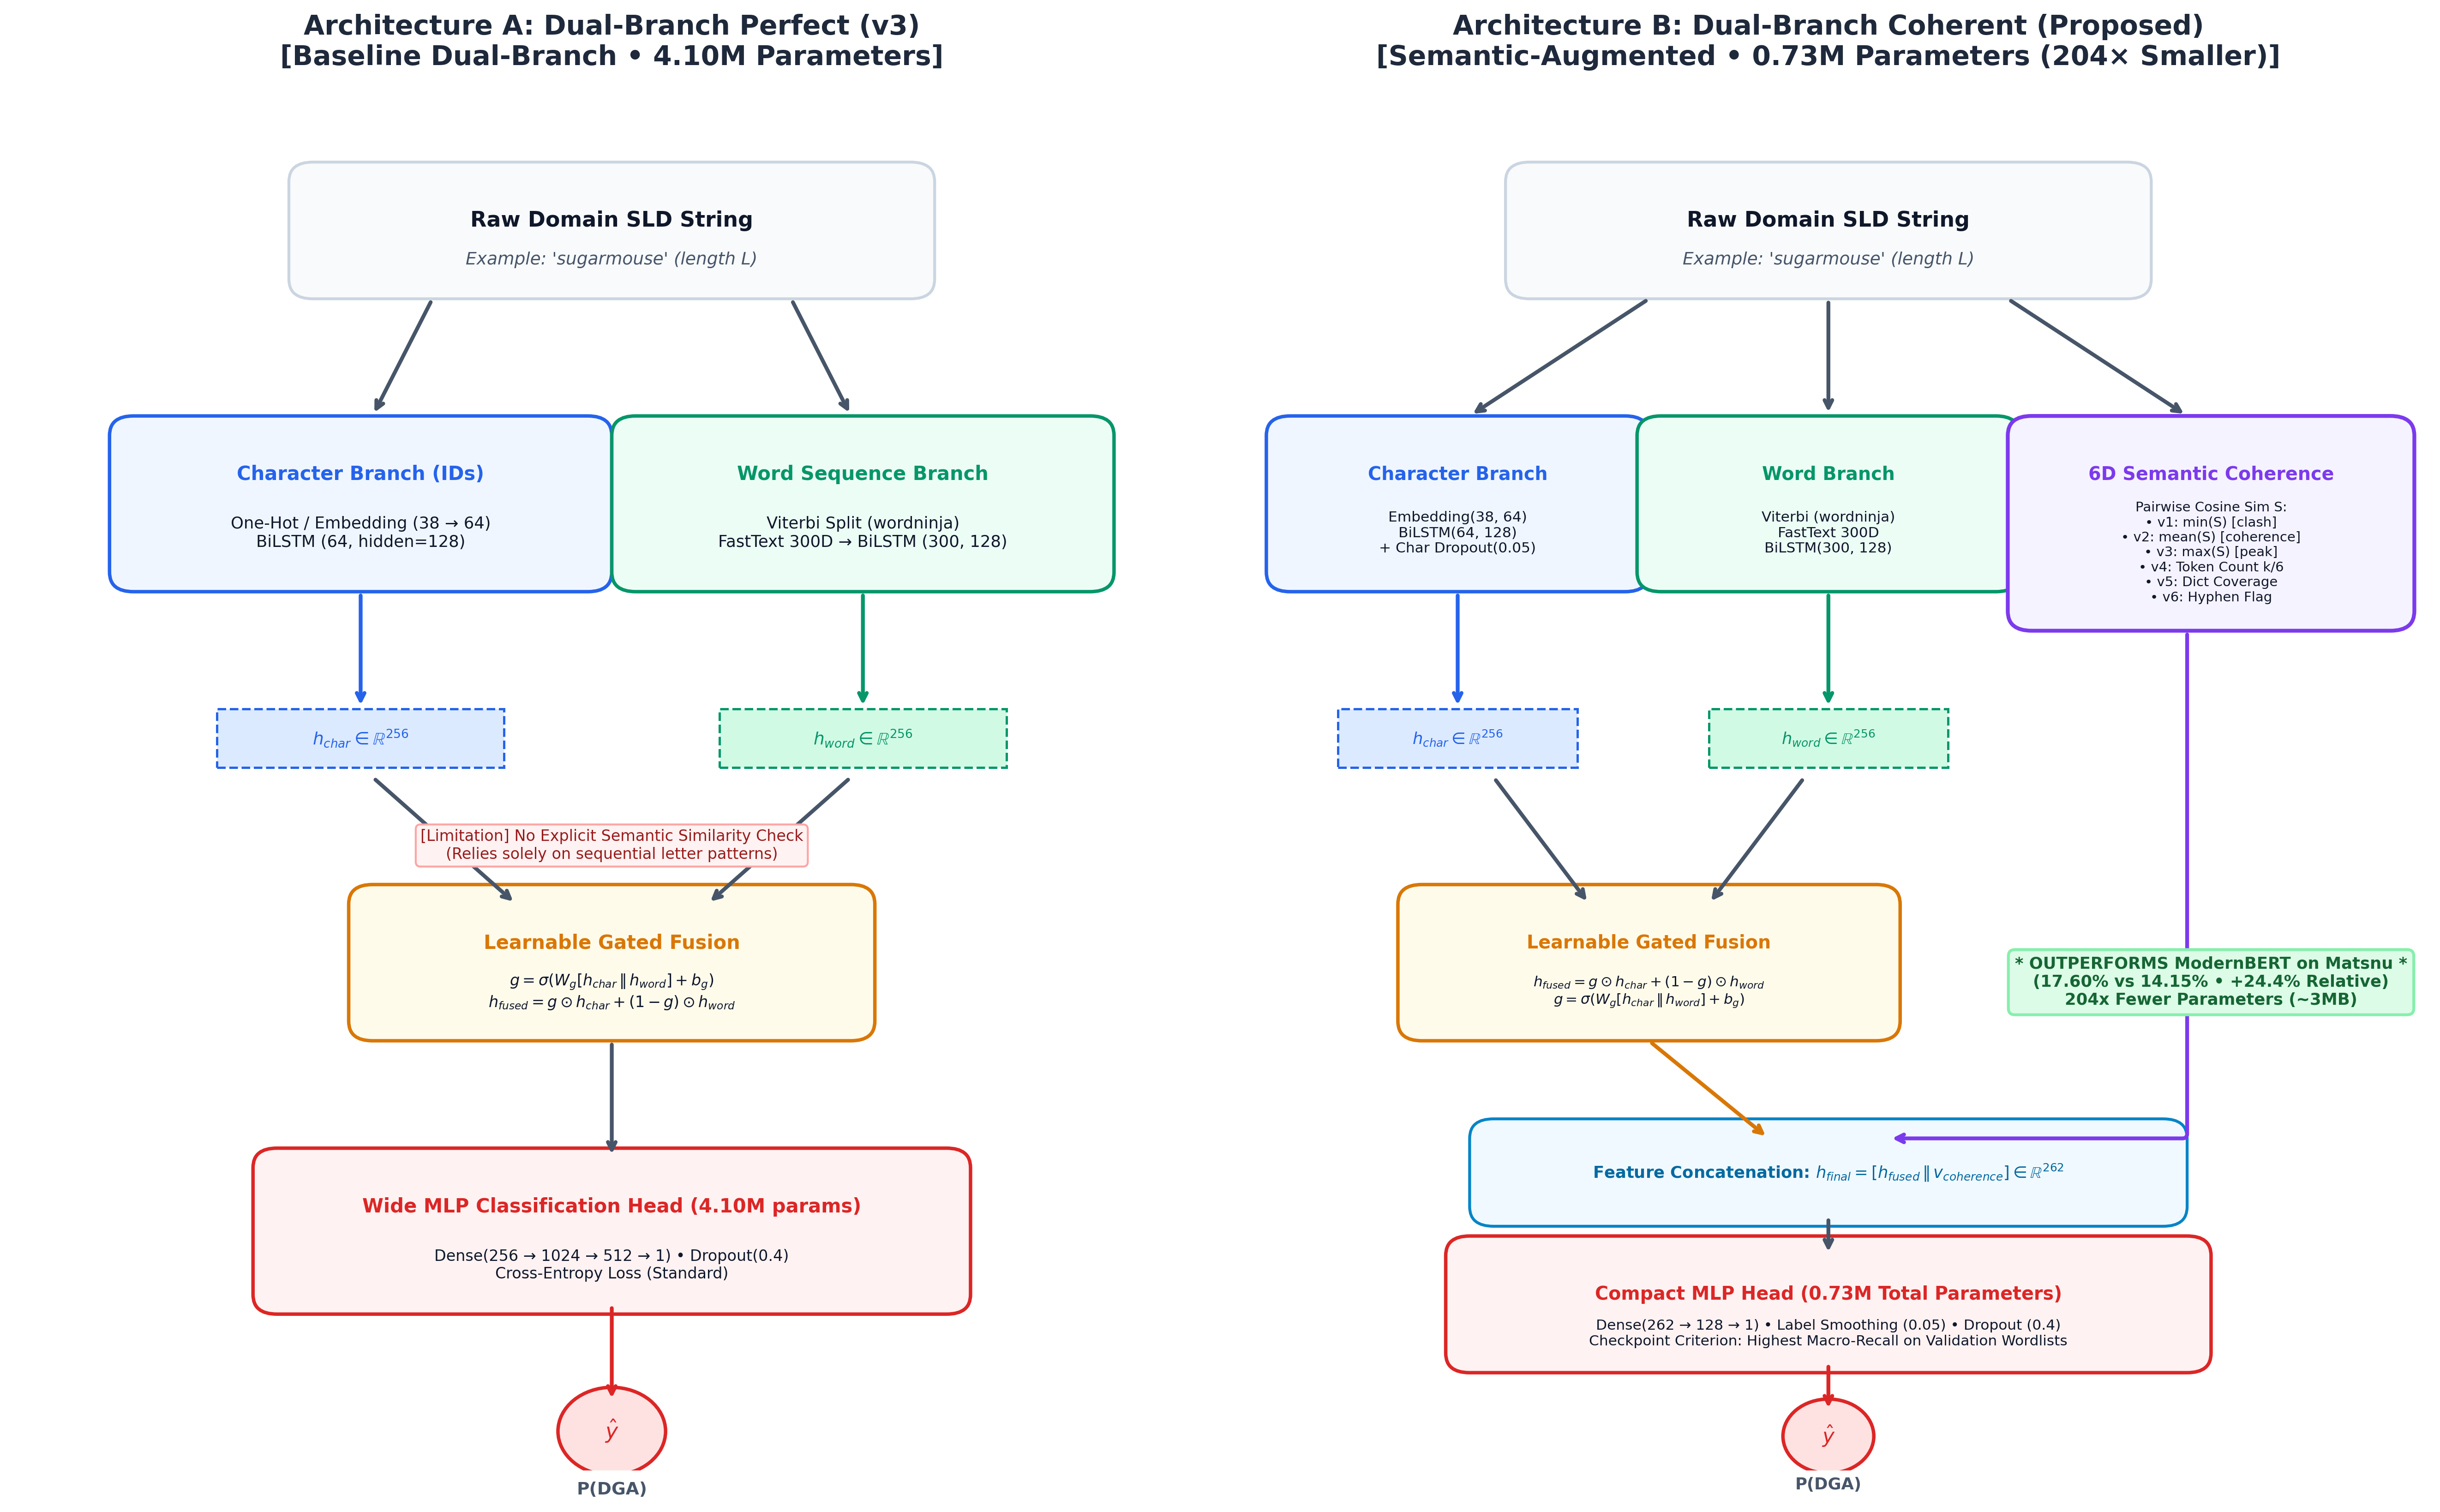
\includegraphics[width=\textwidth]{figures/model_architectures_comparison.png}
\caption{The ablation pair. \emph{Left:} Dual-Branch v3 (4.10M parameters)---character BiLSTM and FastText word-sequence BiLSTM with learnable gated fusion. \emph{Right:} Dual-Branch Coherent (0.73M parameters)---the same backbone with an explicit 6-D semantic coherence vector and a compact head. The coherence vector is computed from frozen embeddings, not learned, so it cannot memorize any family's wordlist.}
\label{fig:arch}
\end{figure*}

\subsection{Ablation control: Dual-Branch v3 (4.10M parameters)}
Identical character and word branches and gated fusion, but no coherence vector and wider projection layers---the architecture that extra \emph{unguided} capacity buys. Trained with the same objective (AdamW, lr $10^{-4}$, weight decay $5{\times}10^{-4}$, dropout 0.5, effective batch 128 via two-step accumulation on a T4, early stopping on the shared criterion).

\subsection{Baselines}
\textbf{Random Forest}---100 trees, class-weighted, over 11 hand-crafted lexical features (entropy, vowel/consonant/digit ratios, bigram commonality, length, and related statistics). \textbf{XGBoost}---the same features, 400 estimators, depth 8, lr 0.05, histogram method. \textbf{ModernBERT-Base}~\cite{modernbert2024} (149M)---BPE-tokenized SLDs (max length 32), fine-tuned on the \emph{full} 1{,}259{,}799-domain training split for 4 epochs (${\sim}39.4$K steps; AdamW lr $3{\times}10^{-5}$, 6\% warmup, FP16, T4), checkpointed on the same criterion. This makes the transformer comparison apples-to-apples: identical data, identical selection metric. \textbf{Soft-voting ensembles}---Ensemble~1 $= 0.5\,p_{\text{BERT}} + 0.5\,p_{\text{v3}}$; Ensemble~2 $= 0.5\,p_{\text{BERT}} + 0.5\,p_{\text{Coherent}}$.

\section{Experimental Setup}
All deep models were trained on Kaggle Tesla T4 (16 GB) notebooks with seed 42 fixed across Python/NumPy/PyTorch; classical baselines on local CPU/RTX~3050. The frozen test set (10{,}000 DGA across five unseen families at 2{,}000 each, plus 9{,}998 unseen benign domains) was scored once at threshold $\tau = 0.50$ with accuracy, balanced accuracy, precision, recall, specificity, FPR, binary and macro F1, MCC, ROC-AUC, PR-AUC, and per-family recall. The complete machine-readable metrics, LaTeX tables, and 300-DPI figures are committed alongside this paper's artifacts, with a script that recomputes every reported number.

\section{Results}
\label{sec:results}
\subsection{Master benchmark}
Table~\ref{tab:master} reports the frozen test-unseen benchmark. Every deep model clears the confirmed zero-day floor of Drichel et al.~\cite{drichel2022} (19.4\% F1, leave-one-cluster-out across all DGArchive families) by a wide margin, and none approaches the wordlist-trained ceiling of~\cite{leyva2026} (80.9--84.6\% F1)---the distance between those two numbers is, in large part, the cost of blindness to the dictionary, which is the point of the benchmark. Anchor figures use different metrics and family mixes and are contextual, not exact comparisons (Section~\ref{sec:limitations}); the defensible comparisons are internal to this protocol.

\begin{table*}[t]
\centering
\caption{Master benchmark on the frozen test-unseen split (19{,}998 domains; $\tau = 0.50$). WL = wordlist; zero-shot WL = recall on \texttt{ngioweb}+\texttt{pizd}, the families genuinely held out by [2]. Bold marks the best value per column.}
\label{tab:master}
\footnotesize
\setlength{\tabcolsep}{4.5pt}
\begin{tabular}{@{}lrrrrrrrrr@{}}
\toprule
Model & Params & Zero-shot WL & \texttt{matsnu} (hard) & WL macro & Non-WL macro & Benign spec. & F1 & ROC-AUC & PR-AUC \\
\midrule
Random Forest & --- & 12.88\% & 9.25\% & 11.67\% & 93.45\% & 82.68\% & 0.5489 & 0.6771 & 0.7335 \\
XGBoost & --- & 9.93\% & 0.95\% & 6.93\% & 94.03\% & 86.18\% & 0.5369 & 0.6577 & 0.7315 \\
Dual-Branch v3 & 4.10M & 30.50\% & 15.70\% & 25.57\% & 99.93\% & 85.55\% & 0.6516 & 0.7440 & 0.8059 \\
Dual-Branch Coherent & 0.73M & 37.75\% & \textbf{17.60\%} & 31.03\% & 99.95\% & 86.23\% & 0.6799 & 0.7671 & 0.8239 \\
ModernBERT-Base & 149.0M & \textbf{45.45\%} & 14.15\% & \textbf{35.02\%} & 99.90\% & \textbf{95.56\%} & \textbf{0.7372} & \textbf{0.8330} & \textbf{0.8787} \\
Ensemble 1 (BERT+v3) & 153.1M & 42.93\% & 12.80\% & 32.88\% & 99.98\% & 94.84\% & 0.7244 & 0.7977 & 0.8550 \\
Ensemble 2 (BERT+Coh) & 149.7M & 44.35\% & 14.05\% & 34.25\% & \textbf{100.00\%} & 94.88\% & 0.7310 & 0.8085 & 0.8624 \\
\bottomrule
\end{tabular}
\end{table*}

\subsection{Per-family recall}
Table~\ref{tab:family} decomposes recall by the five zero-day families. Classical models collapse uniformly. ModernBERT leads on the hyphen-delimited families (\texttt{ngioweb}: 68.25\%, \texttt{pizd}: 22.65\%) but falls to 14.15\% on \texttt{matsnu}; Dual-Branch Coherent overtakes it exactly there (17.60\%) while remaining within 11 points on \texttt{ngioweb}.

\begin{table}[t]
\centering
\caption{Per-family recall (\%) on the frozen test split (2{,}000 domains per family); the last column is benign specificity. WL = wordlist.}
\label{tab:family}
\scriptsize
\setlength{\tabcolsep}{3.6pt}
\begin{tabular}{@{}lrrrrrr@{}}
\toprule
Model & \texttt{ngioweb} & \texttt{pizd} & \texttt{matsnu} & \texttt{tinba} & \texttt{murofet} & benign \\
\midrule
Rand.\ Forest & 9.10 & 16.65 & 9.25 & 93.85 & 93.05 & 82.68 \\
XGBoost & 6.30 & 13.55 & 0.95 & 94.85 & 93.20 & 86.18 \\
Dual v3 & 49.85 & 11.15 & 15.70 & 99.90 & 99.95 & 85.55 \\
Dual Coherent & 57.10 & 18.40 & \textbf{17.60} & 99.90 & \textbf{100.00} & 86.23 \\
ModernBERT & \textbf{68.25} & \textbf{22.65} & 14.15 & 99.85 & 99.95 & \textbf{95.56} \\
Ensemble 1 & 66.40 & 19.45 & 12.80 & \textbf{100.00} & 99.95 & 94.84 \\
Ensemble 2 & 68.30 & 20.40 & 14.05 & \textbf{100.00} & \textbf{100.00} & 94.88 \\
\bottomrule
\end{tabular}
\end{table}

\begin{figure}[t]
\centering
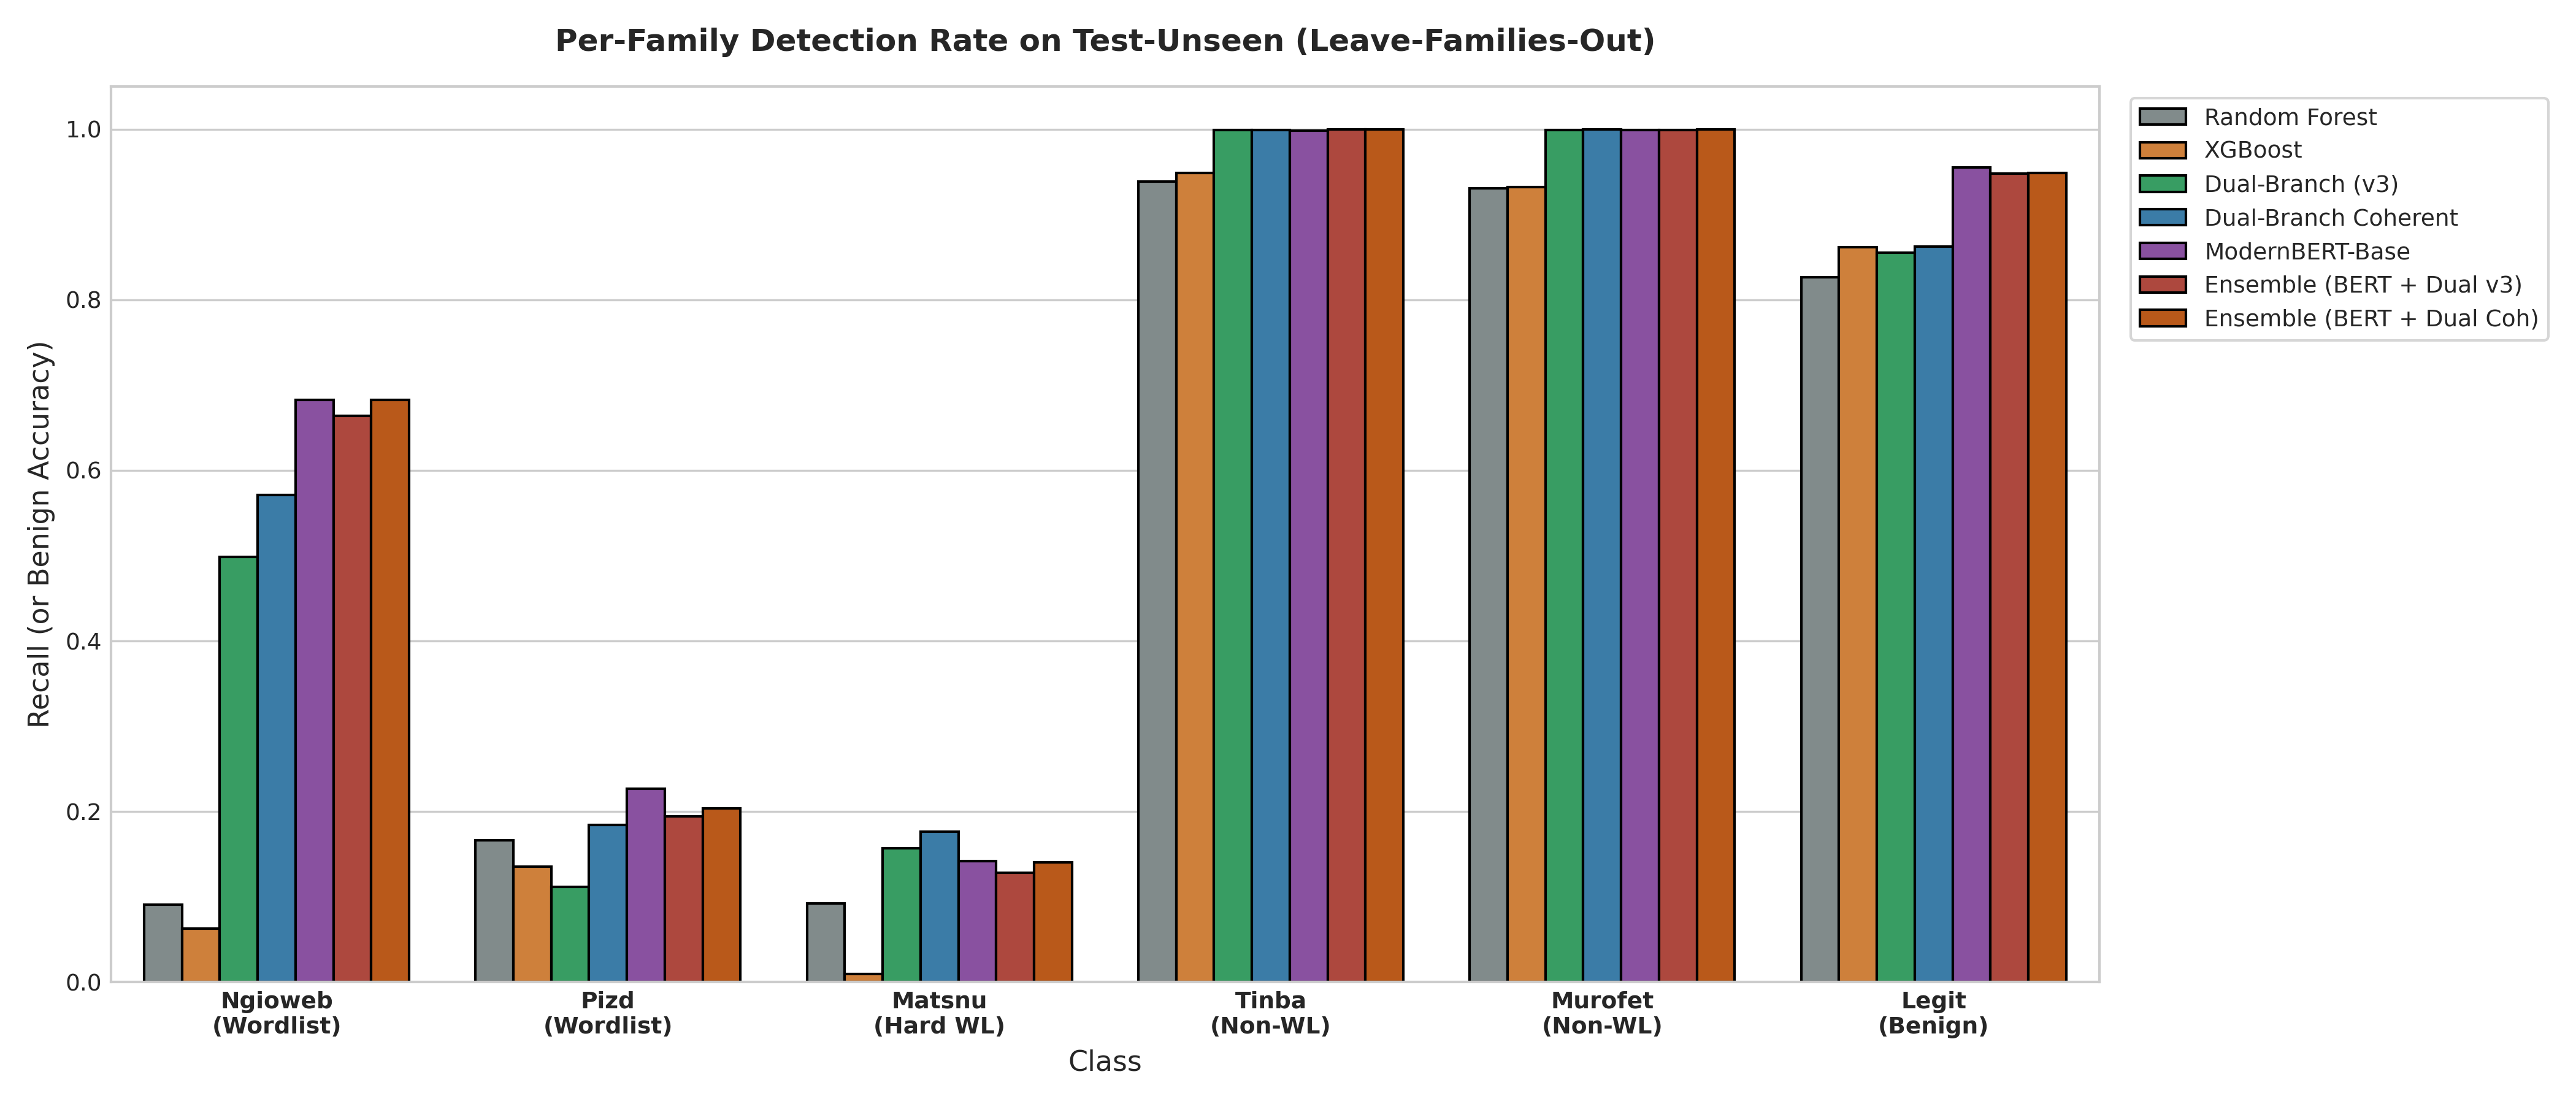
\includegraphics[width=\columnwidth]{figures/fig4_per_family_recall_barchart.png}
\caption{The \texttt{matsnu} inversion: ModernBERT leads on the hyphen-delimited families (\texttt{ngioweb}, \texttt{pizd}) but is overtaken by Dual-Branch Coherent on \texttt{matsnu}---the one family whose words are concatenated with no delimiter.}
\label{fig:inversion}
\end{figure}

\subsection{Checkpoint robustness: validation vs.\ frozen test}
Table~\ref{tab:valtest} compares validation and test performance. Classical models lose 9--10 points of wordlist recall on genuinely unseen families, whereas both semantic models \emph{improve} (Coherent $+2.58$, ModernBERT $+8.97$). A model that memorized validation-family vocabulary would be expected to regress; the observed gains indicate that checkpointing on held-out wordlist recall selects transferable lexical--semantic structure.

\begin{table}[t]
\centering
\caption{Validation-unseen vs.\ frozen test-unseen performance (checkpoint robustness).}
\label{tab:valtest}
\footnotesize
\setlength{\tabcolsep}{3.5pt}
\begin{tabular}{@{}lrrrr@{}}
\toprule
& \multicolumn{2}{c}{WL macro recall} & \multicolumn{2}{c}{F1} \\
\cmidrule(lr){2-3}\cmidrule(lr){4-5}
Model & Val & Test & Val & Test \\
\midrule
Random Forest & 21.77\% & 11.67\% ($-10.10$) & 0.5961 & 0.5489 \\
XGBoost & 16.17\% & 6.93\% ($-9.24$) & 0.5839 & 0.5369 \\
Dual-Branch v3 & 24.80\% & 25.57\% ($+0.77$) & 0.6410 & 0.6516 \\
Dual-Branch Coherent & 28.45\% & 31.03\% ($+2.58$) & 0.6710 & 0.6799 \\
ModernBERT-Base & 26.05\% & 35.02\% ($+8.97$) & 0.6493 & 0.7372 \\
\bottomrule
\end{tabular}
\end{table}

\section{Analysis}
\subsection{The coherence vector is a genuine ablation gain}
Dual-Branch v3 and Coherent share branches, fusion, and training protocol; the only differences are the 6-D vector and a narrower head. Adding the vector---while \emph{removing} 3.37M parameters of projection width---raises wordlist macro-recall from 25.57\% to 31.03\% ($+5.46$ points, $+21.4\%$ relative), \texttt{matsnu} recall from 15.70\% to 17.60\%, \texttt{ngioweb} recall from 49.85\% to 57.10\%, binary F1 from 0.6516 to 0.6799, and ROC-AUC from 0.7440 to 0.7671. A gain produced by a smaller network cannot be attributed to capacity: the computed semantic signal supplies information the unguided parameters could not. The improvement also spans families rather than fitting one outlier, indicating the vector generalizes across wordlist dictionaries instead of overfitting one.

\subsection{The \texttt{matsnu} inversion and subword fluency}
\label{sec:inversion}
On \texttt{matsnu}, Dual-Branch Coherent detects 352/2{,}000 (17.60\%) against ModernBERT's 283/2{,}000 (14.15\%)---a $+24.4\%$ relative gain at $204\times$ fewer parameters (Fig.~\ref{fig:inversion}). The mechanism is architectural. ModernBERT's BPE tokenizer decomposes \texttt{sugarmouse} into frequent, individually grammatical subwords; self-attention over fluent fragments yields a high language-plausibility score and a benign verdict. \texttt{wordninja} recovers the same headwords, but the coherence vector evaluates them in FastText space, where randomly selected dictionary words have near-zero pairwise similarity; the vector registers semantic disharmony ($\min(S) \to 0$) and the gate routes detection accordingly. The effect is specific to the unseparated case: on hyphen-delimited \texttt{ngioweb}/\texttt{pizd}, ModernBERT's web-scale model of legitimate naming dominates (68.25\%/22.65\% vs.\ 57.10\%/18.40\%). Subword fluency, in other words, is a measurable blind spot with a measurable remedy---not a general verdict on transformers, which win every aggregate metric in Table~\ref{tab:master}.

\subsection{Cross-branch mechanism analysis}
The fusion gate is this architecture's interpretable cross-branch mechanism: $g$ is the learned trust in the character branch and $1-g$ the trust in the word/coherence path (there is no attention module whose weights could be inspected instead). The executed training runs record gate statistics on the validation-unseen split (Table~\ref{tab:gate}). In the ablation run (v3), the gate is nearly uniform across input classes (0.183--0.230)---the run log itself flagged that the gate had not learned to differentiate. In the proposed model the gate sharpens: on algorithmic (non-wordlist) domains trust collapses onto the character branch ($g = 0.100$), while wordlist and benign domains---where character statistics are uninformative by construction---retain the word/coherence path ($g \approx 0.25$). The coherence branch therefore does not merely add a feature; it changes what the fusion layer learns to do.

\begin{table}[t]
\centering
\caption{Mean fusion-gate value $g$ (character-branch trust) on the validation-unseen split, recorded in the executed training runs.}
\label{tab:gate}
\footnotesize
\setlength{\tabcolsep}{4pt}
\begin{tabular}{@{}lrr@{}}
\toprule
Input class & Dual-Branch v3 & Dual-Branch Coherent \\
\midrule
Overall & 0.195 & 0.210 \\
Wordlist DGA (val families) & 0.230 & 0.248 \\
Non-wordlist DGA (val families) & 0.183 & 0.100 \\
Benign & --- & 0.246 \\
\bottomrule
\end{tabular}
\end{table}

The coherence vector behaves as hypothesized in the recorded case studies from the executed run: legitimate compounds span mildly positive minimum pairwise similarity (0.07--0.22: \texttt{fishing-shop} 0.22, \texttt{thebankroll} 0.12, \texttt{apple-tshirt} 0.07), while dictionary-DGA concatenations from four different families cluster near zero (\texttt{sugar-claim-mouse} $-0.02$, \texttt{fieldmarry} 0.01, \texttt{reportboringassumption} 0.01, \texttt{applefriends} 0.09). The two distributions overlap on individual examples---as expected of a statistical signal rather than a rule---but their mass is shifted, and the shift is family-independent: the same \texttt{sugarmouse} that reads as fluent English to a BPE tokenizer is near-orthogonal in FastText space.

\subsection{Operational trade-offs}
In an SOC, false positives page humans; every count in this subsection is an operating point at the default threshold $\tau = 0.50$. ModernBERT produces 444 false positives on 9{,}998 benign domains (95.56\% specificity; MCC 0.6025) versus 1{,}377 for Coherent (86.23\%)---a direct consequence of billions of web tokens that let it recognize real brand blends (\texttt{techradar}, \texttt{ticketmaster}) a small network flags as anomalous. Ensemble 2 blends both signals and delivers the deployment profile: 100.00\% recall on unseen non-wordlist families, 94.88\% specificity (512 false alarms), 34.25\% wordlist macro-recall, ROC-AUC 0.8085. The threshold trade-off (wordlist recall vs.\ benign specificity across $\tau \in [0.01, 0.99]$) is released with the artifacts (Fig.~\ref{fig:threshold}). Because findings about false alarms and deployment profiles are operating-point statements, the executed runs also record a decision-threshold sweep on the validation-unseen split (Table~\ref{tab:threshold}). Two conclusions survive the sweep. First, ModernBERT's specificity advantage is not an artifact of $\tau = 0.50$: at matched benign accuracy ${\approx}\,0.92$ it reaches 0.338 validation wordlist macro-recall, whereas Coherent attains a comparable 0.465 only by conceding benign accuracy 0.751. Second, Coherent's wordlist recall is strongly recoverable by lowering the threshold (0.348 $\to$ 0.661 from $\tau = 0.50$ to $0.15$) at a real specificity cost. The SOC-relevant statement is therefore not a single ranking but the shape of the recall/specificity frontier (Fig.~\ref{fig:threshold}), on which Ensemble~2 remains the balanced operating point.

\begin{table}[t]
\centering
\caption{Operating-point robustness: decision-threshold sweep on the validation-unseen split, recorded in the executed training runs.}
\label{tab:threshold}
\footnotesize
\setlength{\tabcolsep}{4.5pt}
\begin{tabular}{@{}lrrrr@{}}
\toprule
& \multicolumn{2}{c}{Dual-Branch Coherent} & \multicolumn{2}{c}{ModernBERT-Base} \\
\cmidrule(lr){2-3}\cmidrule(lr){4-5}
$\tau$ & WL macro & Benign acc. & WL macro & Benign acc. \\
\midrule
0.50 & 0.348 & 0.860 & 0.261 & 0.954 \\
0.30 & 0.465 & 0.751 & 0.338 & 0.924 \\
0.15 & 0.661 & 0.520 & 0.424 & 0.875 \\
\bottomrule
\end{tabular}
\end{table}

\begin{figure}[t]
\centering
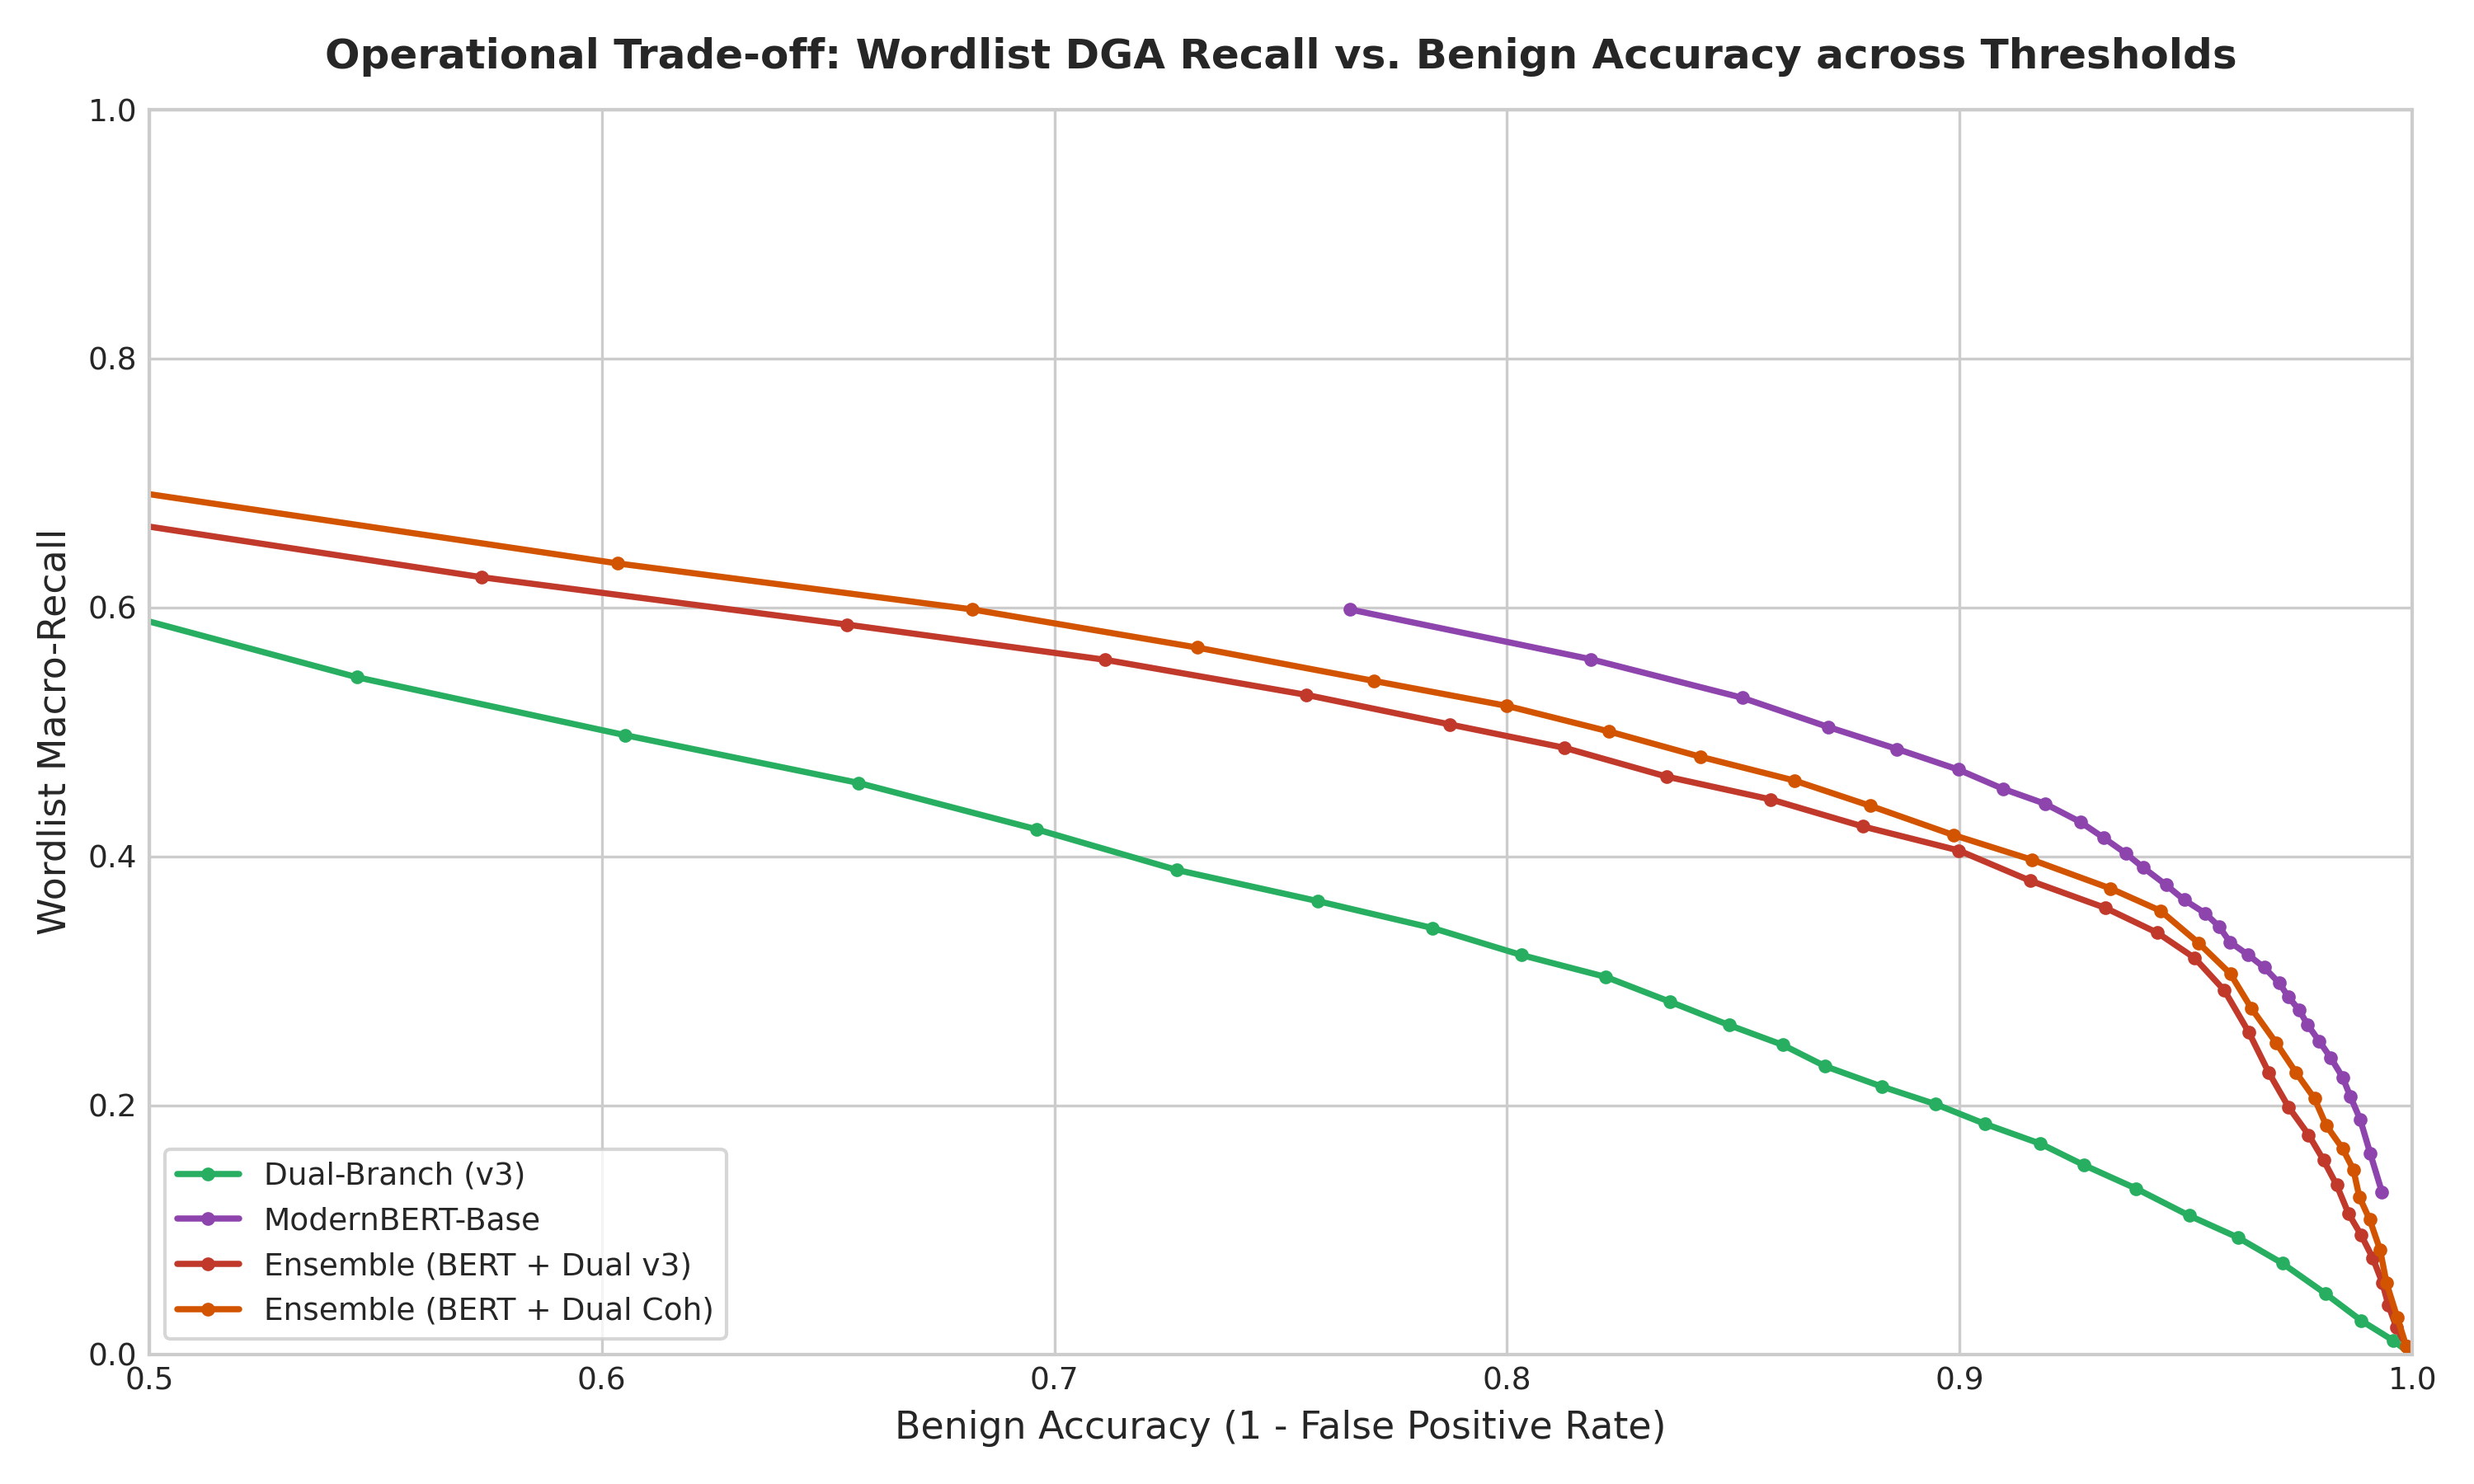
\includegraphics[width=\columnwidth]{figures/fig6_threshold_tradeoff_curves.png}
\caption{Operational trade-off: wordlist macro-recall vs.\ benign specificity as the decision threshold varies. All reported tables use $\tau = 0.50$.}
\label{fig:threshold}
\end{figure}

\subsection{Efficiency per parameter}
Normalizing wordlist macro-recall by model size makes the cost/benefit explicit (Table~\ref{tab:efficiency}): Coherent delivers ${\sim}180\times$ ModernBERT's wordlist recall per million parameters at ${\sim}3$ MB vs.\ ${\sim}570$ MB of weights. The BiLSTM stack is a CPU-viable design for recursive resolvers, forward proxies, and edge firewalls; we make no measured latency claim beyond this deployment profile, which a 149M transformer requiring GPU batching cannot match. The two models occupy genuinely different points on the accuracy/cost curve---which is precisely why their ensemble dominates either alone on the balanced deployment metrics above.

\begin{table}[t]
\centering
\caption{Wordlist macro-recall per million parameters (Recall/M).}
\label{tab:efficiency}
\footnotesize
\setlength{\tabcolsep}{5pt}
\begin{tabular}{@{}lrrr@{}}
\toprule
Model & Params & WL macro & Recall/M \\
\midrule
Dual Coherent & 0.73M & 31.03\% & 42.51 \\
Dual v3 & 4.10M & 25.57\% & 6.24 \\
ModernBERT & 149.0M & 35.02\% & 0.24 \\
\bottomrule
\end{tabular}
\end{table}

\section{Limitations and Threats to Validity}
\label{sec:limitations}
\textbf{Scope of blind families.} Only three wordlist families are truly blind test cases. This is stronger than single-family designs but small; per-family results should be read as case studies, not a statistically robust average. \textbf{\texttt{matsnu} is one family.} The inversion is a targeted finding on the hardest unseparated-dictionary case, not a claim of general transformer inferiority---ModernBERT wins every aggregate metric. \textbf{\texttt{manuelita} is a validation diagnostic}, not a blind score; this trades a clean one-shot number for an actionable read during training, and is disclosed rather than hidden. \textbf{Anchor comparability.} The 19.4\% floor~\cite{drichel2022} is leave-one-cluster-out F1 across all DGArchive families and the 80.9\% ceiling~\cite{leyva2026} is F1 measured with eight wordlist families in training; our headline metrics are recall on a different family mix. Cross-study numbers are contextual; the internally consistent comparisons are those within this protocol, and the family-matched \texttt{ngioweb}/\texttt{pizd} comparison. \textbf{Deterministic data.} UMUDGA domains are generated by executing each family's DGA with fixed seeds---realistic strings, but absent live-traffic properties such as registration timing. \textbf{Benign difficulty.} Alexa/Tranco top domains are structurally ``easy'' negatives; production false-positive rates will be worse than measured here. \textbf{Segmentation and coverage.} \texttt{wordninja}'s unigram segmentation can err on rare, compressed, or multilingual concatenations, degrading the coherence vector; FastText is English-centric, so IDNs and non-English wordlist families require multilingual embedding spaces. \textbf{Threshold.} All test-set results use $\tau = 0.50$; deployment requires cost-sensitive calibration. The validation-split sweep (Table~\ref{tab:threshold}) shows the qualitative conclusions survive threshold changes, but exact FP/recall trade-offs are budget-dependent. \textbf{Family provenance.} \texttt{banjori}'s wordlist status is disputed (retained in training); \texttt{charbot} is an adversarially generated family~\cite{peck2019} included for robustness. \textbf{Generality.} Results evidence wordlist-family generalization within this threat model; recent work cautions that models trained on standard corpora generalize poorly to evolving real-world campaigns~\cite{cebere2024}.

\section{Conclusion and Future Work}
Under a fully blind, leak-free Leave-Families-Out benchmark on 1.3M domains, wordlist-DGA zero-day detection remains far from solved: a fine-tuned 149M ModernBERT reaches 35.02\% wordlist macro-recall and collapses to 14.15\% on unseparated dictionary words. The proposed Dual-Branch Coherent architecture---0.73M parameters, with an explicit, computed semantic-coherence vector---beats the transformer on exactly that failure mode (+24.4\% relative) while delivering ${\sim}180\times$ more wordlist recall per parameter, and the two signals combine in an ensemble that offers the strongest deployment profile. The broader methodological contribution stands regardless of architecture: published wordlist-DGA scores measured with the malware's dictionary in training overstate zero-day readiness, and blind evaluation collapses them. Future work will extend the coherence signal with multilingual embedding spaces, evaluate adversarial robustness (homoglyph and insertion attacks) against both branches, fuse passive-DNS context (TTL, IP reputation, registration recency), replace the scalar gate with attention-based fusion, and grow the set of blind wordlist families toward a standardized public benchmark.

\section*{Artifact Availability}
The complete research artifact---dataset construction pipeline, all executed training and evaluation notebooks with outputs, machine-readable metrics, LaTeX/CSV tables, 300-DPI figures, and a verification script that recomputes every number in this paper---is available at \url{https://github.com/WalidMahmood/dga-detection-generalization}. Model weights and the merged corpus are redistributable from their public sources.

\begin{thebibliography}{15}

\bibitem{plohmann2016}
D. Plohmann, K. Yakdan, M. Klatt, J. Bader, and E. Gerhards-Padilla, ``A comprehensive measurement study of domain generating malware,'' in \emph{Proc. 25th USENIX Security Symposium}, 2016, pp. 263--278.

\bibitem{leyva2026}
R. Leyva La O, C. A. Catania, and R. Gonzalez, ``Expert selection for wordlist-based DGA detection,'' \emph{IEEE Latin America Transactions}, vol. 24, no. 1, pp. 33--42, 2026.

\bibitem{drichel2022}
A. Drichel, T. Meuser, and U. Meyer, ``On the evaluation of DGA detectors,'' in \emph{Proc. 25th Int. Symp. Research in Attacks, Intrusions and Defenses (RAID)}, 2022, pp. 1--15.

\bibitem{modernbert2024}
B. Warner, A. Chaffin, B. Clavi\'e, O. Weller, O. Hallstr\"om, S. Taghadouini, A. Gallagher, R. Biswas, F. Ladhak, T. Aarsen, N. Cooper, and J. Howard, ``Smarter, better, faster, longer: A modern bidirectional encoder for fast, memory efficient, and long context finetuning and inference,'' arXiv:2412.13663, 2024.

\bibitem{bilge2011}
L. Bilge, E. Kirda, C. Kruegel, and M. Balduzzi, ``EXPOSURE: Finding malicious domains using passive DNS analysis,'' in \emph{Proc. NDSS}, 2011.

\bibitem{antonakakis2012}
M. Antonakakis et al., ``From throw-away traffic to bots: Detecting the rise of DGA-based malware,'' in \emph{Proc. USENIX Security Symposium}, 2012, pp. 491--506.

\bibitem{schuppen2018}
S. Sch\"uppen, D. Teubert, P. Herrmann, and U. Flegel, ``FANCI: Feature-based automated network analysis for content inspection,'' in \emph{Proc. NDSS}, 2018.

\bibitem{woodbridge2016}
J. Woodbridge, H. S. Anderson, A. Ahuja, and D. Grant, ``Predicting domain generation algorithms with long short-term memory networks,'' arXiv:1611.00791, 2016.

\bibitem{lison2017}
P. Lison and V. Mavroeidis, ``Automatic detection of malware-generated domains with recurrent neural models,'' in \emph{Proc. 10th Norwegian Information Security Conference (NISK)}, 2017. arXiv:1709.07102.

\bibitem{koh2018}
J. J. Koh and B. Rhodes, ``Inline detection of domain generation algorithms with context-sensitive word embeddings,'' in \emph{Proc. IEEE Int. Conf. Big Data}, 2018, pp. 2966--2971.

\bibitem{peck2019}
J. Peck, C. Nie, R. Sivaguru, C. Grumer, F. Olumofin, B. Yu, A. Nascimento, and M. De Cock, ``CharBot: A simple and effective method for evading DGA classifiers,'' in \emph{Proc. RAID}, 2020. arXiv:1905.01078.

\bibitem{cebere2024}
B. Cebere, J. Flueren, S. Sebasti\'an, D. Plohmann, and C. Rossow, ``Down to earth! Guidelines for DGA-based malware detection,'' in \emph{Proc. 27th Int. Symp. Research in Attacks, Intrusions and Defenses (RAID)}, 2024, pp. 147--165.

\bibitem{zago2020dib}
M. Zago, M. Gil P\'erez, and G. Mart\'inez P\'erez, ``UMUDGA: A dataset for profiling algorithmically generated domain names in botnet detection,'' \emph{Data in Brief}, vol. 30, p. 105400, 2020.

\bibitem{zago2020cose}
M. Zago, M. Gil P\'erez, and G. Mart\'inez P\'erez, ``UMUDGA: A dataset for profiling DGA-based botnet,'' \emph{Computers \& Security}, vol. 92, p. 101719, 2020.

\bibitem{bojanowski2017}
P. Bojanowski, E. Grave, A. Joulin, and T. Mikolov, ``Enriching word vectors with subword information,'' \emph{Transactions of the Association for Computational Linguistics}, vol. 5, pp. 135--146, 2017.

\end{thebibliography}

\end{document}
